Convolutional neural networks were first proposed for image
recognition by LeCun et al. \cite{lecun1989backpropagation}, but have
gained wider recognition after the ImageNet 2012
competition \cite{krizhevsky2012imagenet}.  In this work we use 3D
convolutional networks to score protein structures. The architecture
of the model is shown in Fig.\ \ref{Fig:CNNModel}.  It is comprised of
three blocks of alternating convolutional, volumetric batch
normalization, and ReLU layers, followed by three fully-connected
layers with ReLU nonlinearities. The final output of the network is a
single number, interpreted as \tchanged{the} score of the input structure.

\begin{figure}[H]
    \centering
    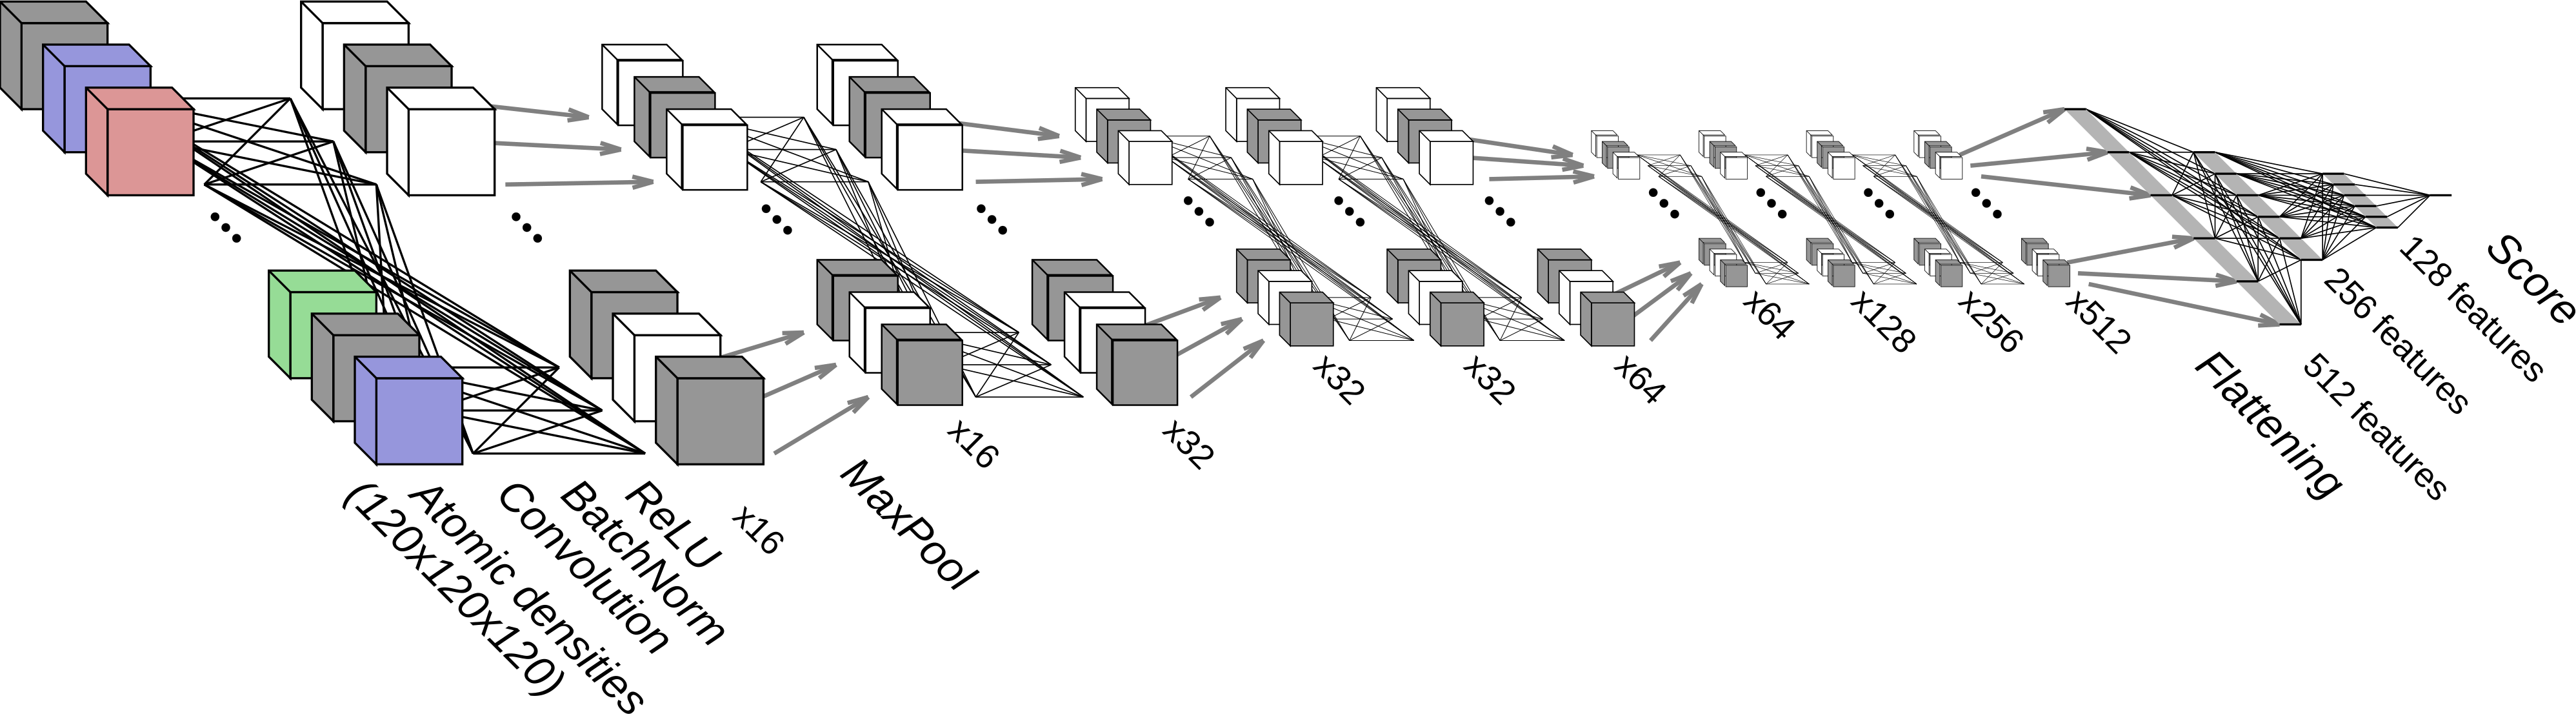
\includegraphics[width=\linewidth]{Fig/ConvnetDiagramV1.eps}

    \caption{Schematic representation of the convolutional neural
    network architecture used in this work.  Line connections across
    boxes denote the consecutive application of a 3D convolutional
    layer (``Convolution''), a batch normalization layer
    (``BatchNorm''), and a ReLU layer. Arrows between boxes denote
    maximum pooling layers (``MaxPool''). The labels ``$\times M$''
    denote the number of filters used in the corresponding 3D
    convolutional layer. The size of all filters and maximum pooling
    domains are $3\times 3\times 3$. The grey stripes denote
    one-dimensional vectors and crossed lines between them stand for
    fully-connected layers with ReLU non-linearities. Details of the
    model parameters can be found in Supplementary Information.}

    \label{Fig:CNNModel}
\end{figure}

Each 3D convolutional layer takes $N$ input density maps $f$ and
transforms them using $M$ filters $F$ according to the following
formula:
%%% GL: I'm replacing \tau by r', just to use a more conventional
%%% notation for convolutions
$$
f^\text{out}_i (\mathbf{r}) = \sum^{N}_{j=1} \int F_i (\mathbf{r} - \mathbf{r'}) \cdot f^\text{in}_j(\mathbf{r'}) ~d\mathbf{r'}, \forall i \in [1,M]
$$
In practice, these convolutions are approximated by sums on a 3D grid.
The ReLU nonlinearity is computed as following:
$$
f^\text{out}_i (\mathbf{r}) = \begin{cases}
               f^\text{in}_i(\mathbf{r}) &\text{if } f^\text{in}_i(\mathbf{r})\geq 0\\
               0                         &\text{if } f^\text{in}_i(\mathbf{r})<0\\
            \end{cases}, \forall i \in [1,M]
$$
The concept of batch normalization layer was introduced by Ioffe and
Szegedy \cite{ioffe2015batch} to address the problem of internal
covariate shift: the change in the distribution of subnetwork outputs
due to the change in its parameters during the training. In practice,
this layer normalizes each input value according to the
mean and variance of the corresponding input within the subset of
examples used to estimate the gradient (``minibatch''):
%%% GL: I'm suggesting to use index k for the minibatch examples
%%% (instead of i, which is already used)
$$
\hat{f}^\text{in}_k(\mathbf{r}) = \frac{f^\text{in}(\mathbf{r}) - \mu_\text{B}}{\sqrt{\sigma^{2}_\text{B} + \epsilon}}, \forall k \in [1,N_\text{B}]
$$
where $\mu_\text{B}(\mathbf{r})
= \frac{1}{N_\text{B}} \sum_{k=1}^{N_\text{B}}
f^\text{in}_i(\mathbf{r})$, and $\sigma^{2}_\text{B}
= \frac{1}{N_\text{B}} \sum_{k=1}^{N_\text{B}} \left(
f^\text{in}_i(\mathbf{r}) - \mu_\text{B}
(\mathbf{r}) \right)^2$. $N_\text{B}$ is the number of examples in the
minibatch. The constant $\epsilon$ is added to avoid division by
zero. Afterwards, the output of this layer is computed by scaling the
normalized inputs:
$$
f^\text{out}_k(\mathbf{r}) = \gamma \hat{f}^\text{in}_k(\mathbf{r}) + \beta, \forall k \in [1,N_B]
$$
The parameters $\gamma$ and $\beta$ are learned along with other
parameters of the network during the training.

The maximum pooling layer (``MaxPool'') is used to build a
coarse-grained representation of the input. The output of this layer
is the maximum over the cubes of size $d \times d \times d$ that cover
the input domain without overlapping.  The output data domain is then
$d$ times smaller than the input data box. All three ``MaxPool''
layers of the model (Fig.\ \ref{Fig:CNNmodel}) use $d=3$.
%%% ??? Why does the size go from 118 to 58?

%%% GL: Should we indicate the size of each grid at each layer? It can
%%% be guessed but it would help the reader if we provide them.

During the coarse-graining procedure, the size of the individual data
grids eventually shrinks to a single cell. The flattening layer
reshapes the array of 3D density maps to a single vector. Afterwards,
we compute several transformations using fully-connected layers. These
layers transform a vector $\mathbf{x}_\text{in}$ as following:
%%% GL: Using the more conventional notation: vectors in bold, matrices in italics
$$
\mathbf{x}_\text{out} = W \cdot \mathbf{x}_\text{in} + \mathbf{b}
$$
where $W$ is a matrix and $\mathbf{b}$ is a vector, learned during the
training.
